\begin{figure}[htbp]
\section*{ TBCK}
\centering
\begin{subfigure}[b]{0.95\textwidth}
\centering
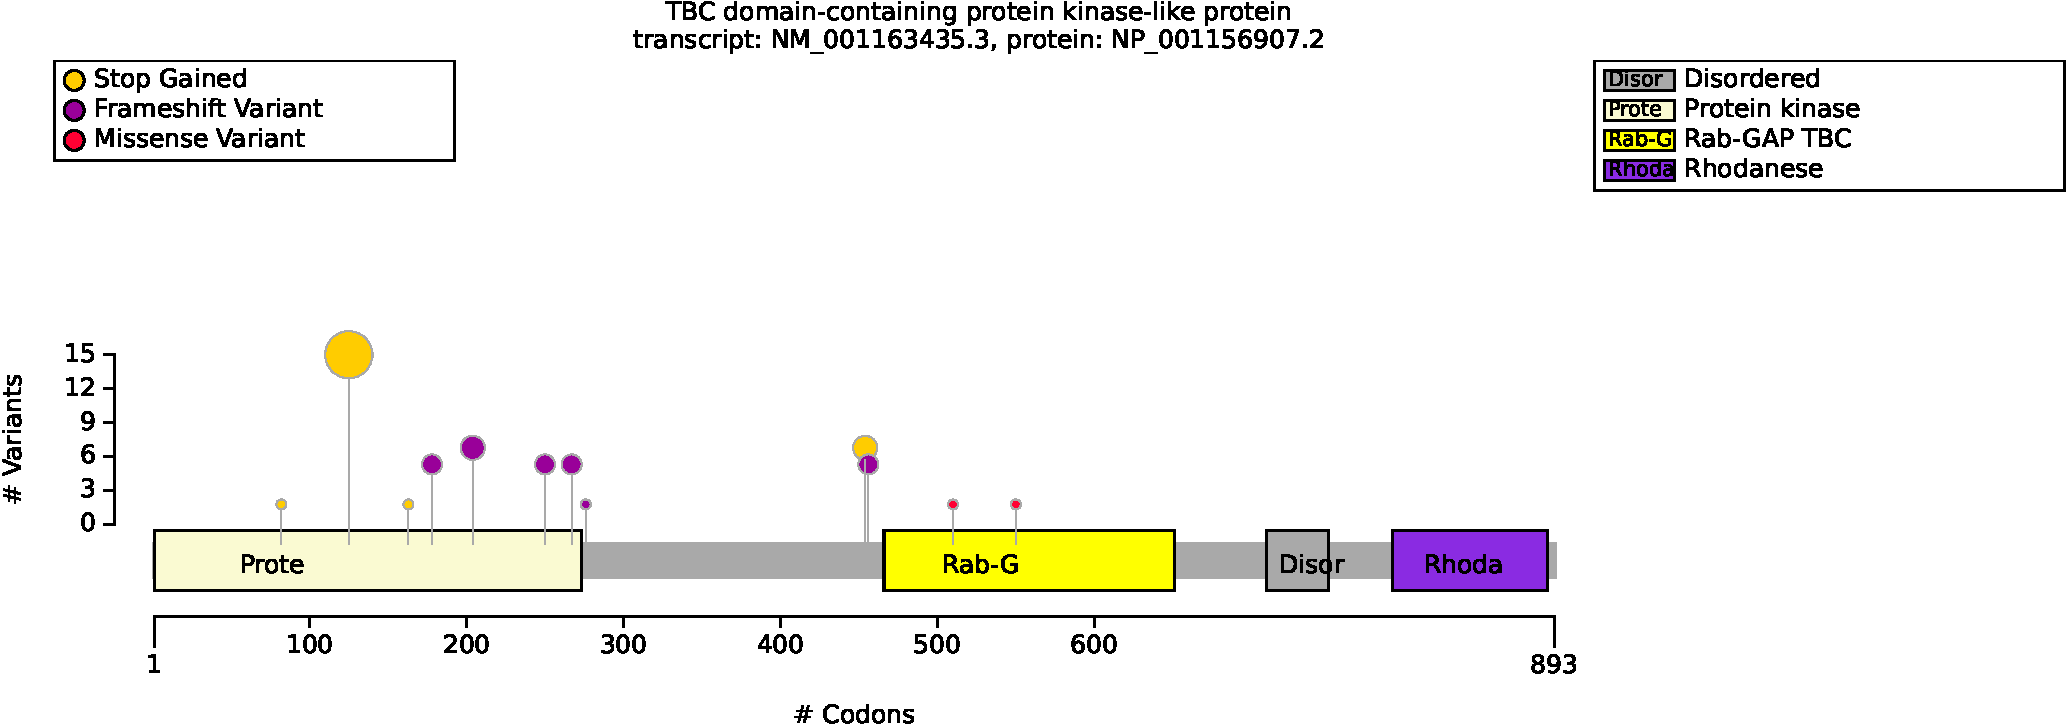
\includegraphics[width=\textwidth]{ img/TBCK_protein_diagram.pdf} 
\captionsetup{justification=raggedright,singlelinecheck=false}
\caption{Distribution of variants in TBCK}
\end{subfigure}

\vspace{2em}

\begin{subfigure}[b]{0.95\textwidth}
\centering
\resizebox{\textwidth}{!}{
\begin{tabular}{llllrr}
\toprule
HPO term & R126*/R126* & R126*/other OR other/other & p-value & adj. p-value\\
\midrule
Macroglossia [HP:0000158] & 11/12 (92\%) & 3/22 (14\%) & $1.34\times 10^{-5}$ & $4.30\times 10^{-4}$\\
Developmental regression [HP:0002376] & 9/12 (75\%) & 2/22 (9\%) & $1.83\times 10^{-4}$ & 0.003\\
\bottomrule
\end{tabular}
}
\captionsetup{justification=raggedright,singlelinecheck=false}
\caption{Fisher Exact Test performed to compare HPO annotation frequency with respect to R126*/R126* and R126*/other OR other/other. Total of
        32 tests were performed.}
\end{subfigure}
\vspace{2em}
\begin{subfigure}[b]{0.95\textwidth}
\centering
\resizebox{\textwidth}{!}{
\begin{tabular}{llllrr}
\toprule
Genotype (A) & Genotype (B) & total tests performed & significant results\\
\midrule
missense/missense OR missense/other & other/other & 30 & 0\\
FEMALE & MALE & 32 & 0\\
\bottomrule
\end{tabular}
}
\captionsetup{justification=raggedright,singlelinecheck=false}
\caption{Fisher Exact Test performed to compare HPO annotation frequency with respect to genotypes.}
\end{subfigure}

\vspace{2em}

\caption{ The cohort comprised 41 individuals (17 females, 24 males). 3 of these individuals were reported to be deceased. A total of 97 HPO terms were used to annotate the cohort. 
Disease diagnosis: Hypotonia, infantile, with psychomotor retardation and characteristic facies 3 (OMIM:616900). 
Durham et al (2023) stated that several studies have touched on a genotype-phenotype correlation of TBCK syndrome; however, more data are required for statistically significant conclusions \cite{PMID_37455236}. 
A total of 18 unique variant alleles were found in \textit{TBCK} (transcript: \texttt{NM\_001163435.3}, protein id: \texttt{NP\_001156907.2}).}
\end{figure}
